% Waste is a problem
% Decisionmakers are contemplating many fuel cycle options
% Decisionmakers are contemplating many repository options
% Interfacing between FCO/SA campaign and UFD campaign

\begin{frame}[ctb!]
  \frametitle{Future Disposal System Options}
   \begin{minipage}{0.44\textwidth}
     \begin{figure}[h!]
         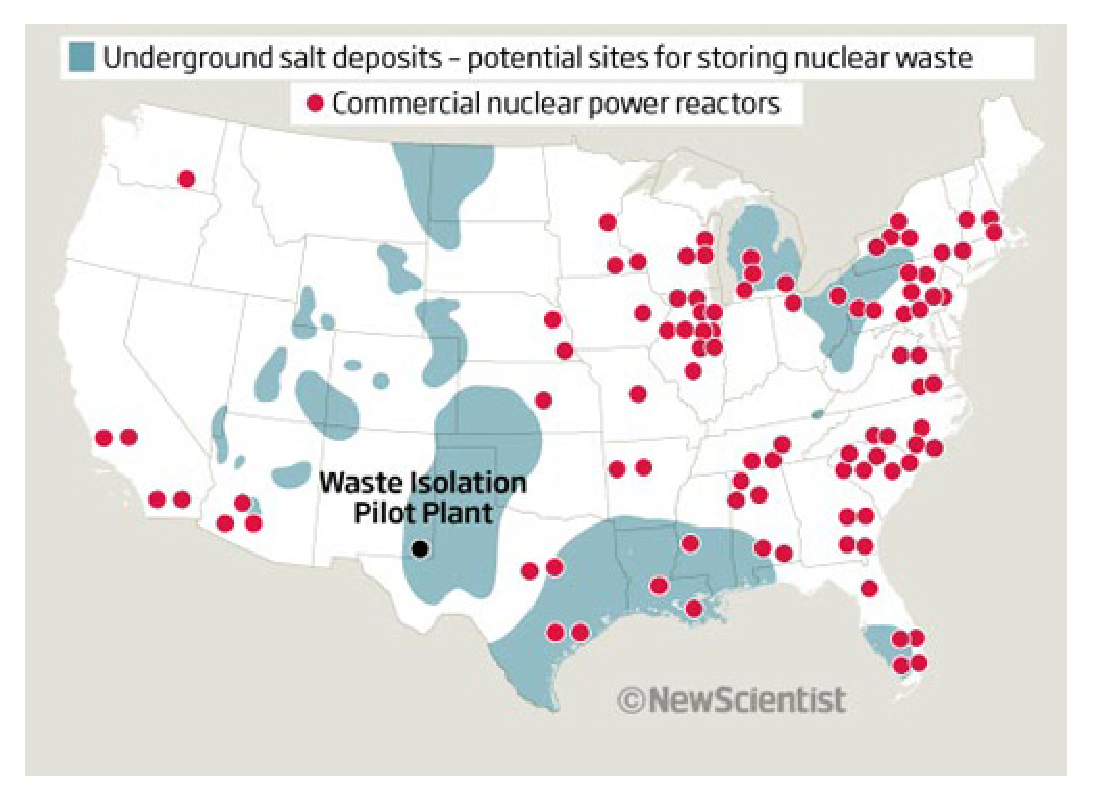
\includegraphics[width=0.8\textwidth]{saltNewScientist.eps}
         \caption{U.S. Salt Deposits, ref. \cite{newscientist_where_2011}.}
     \end{figure}
     \begin{figure}[h!]
         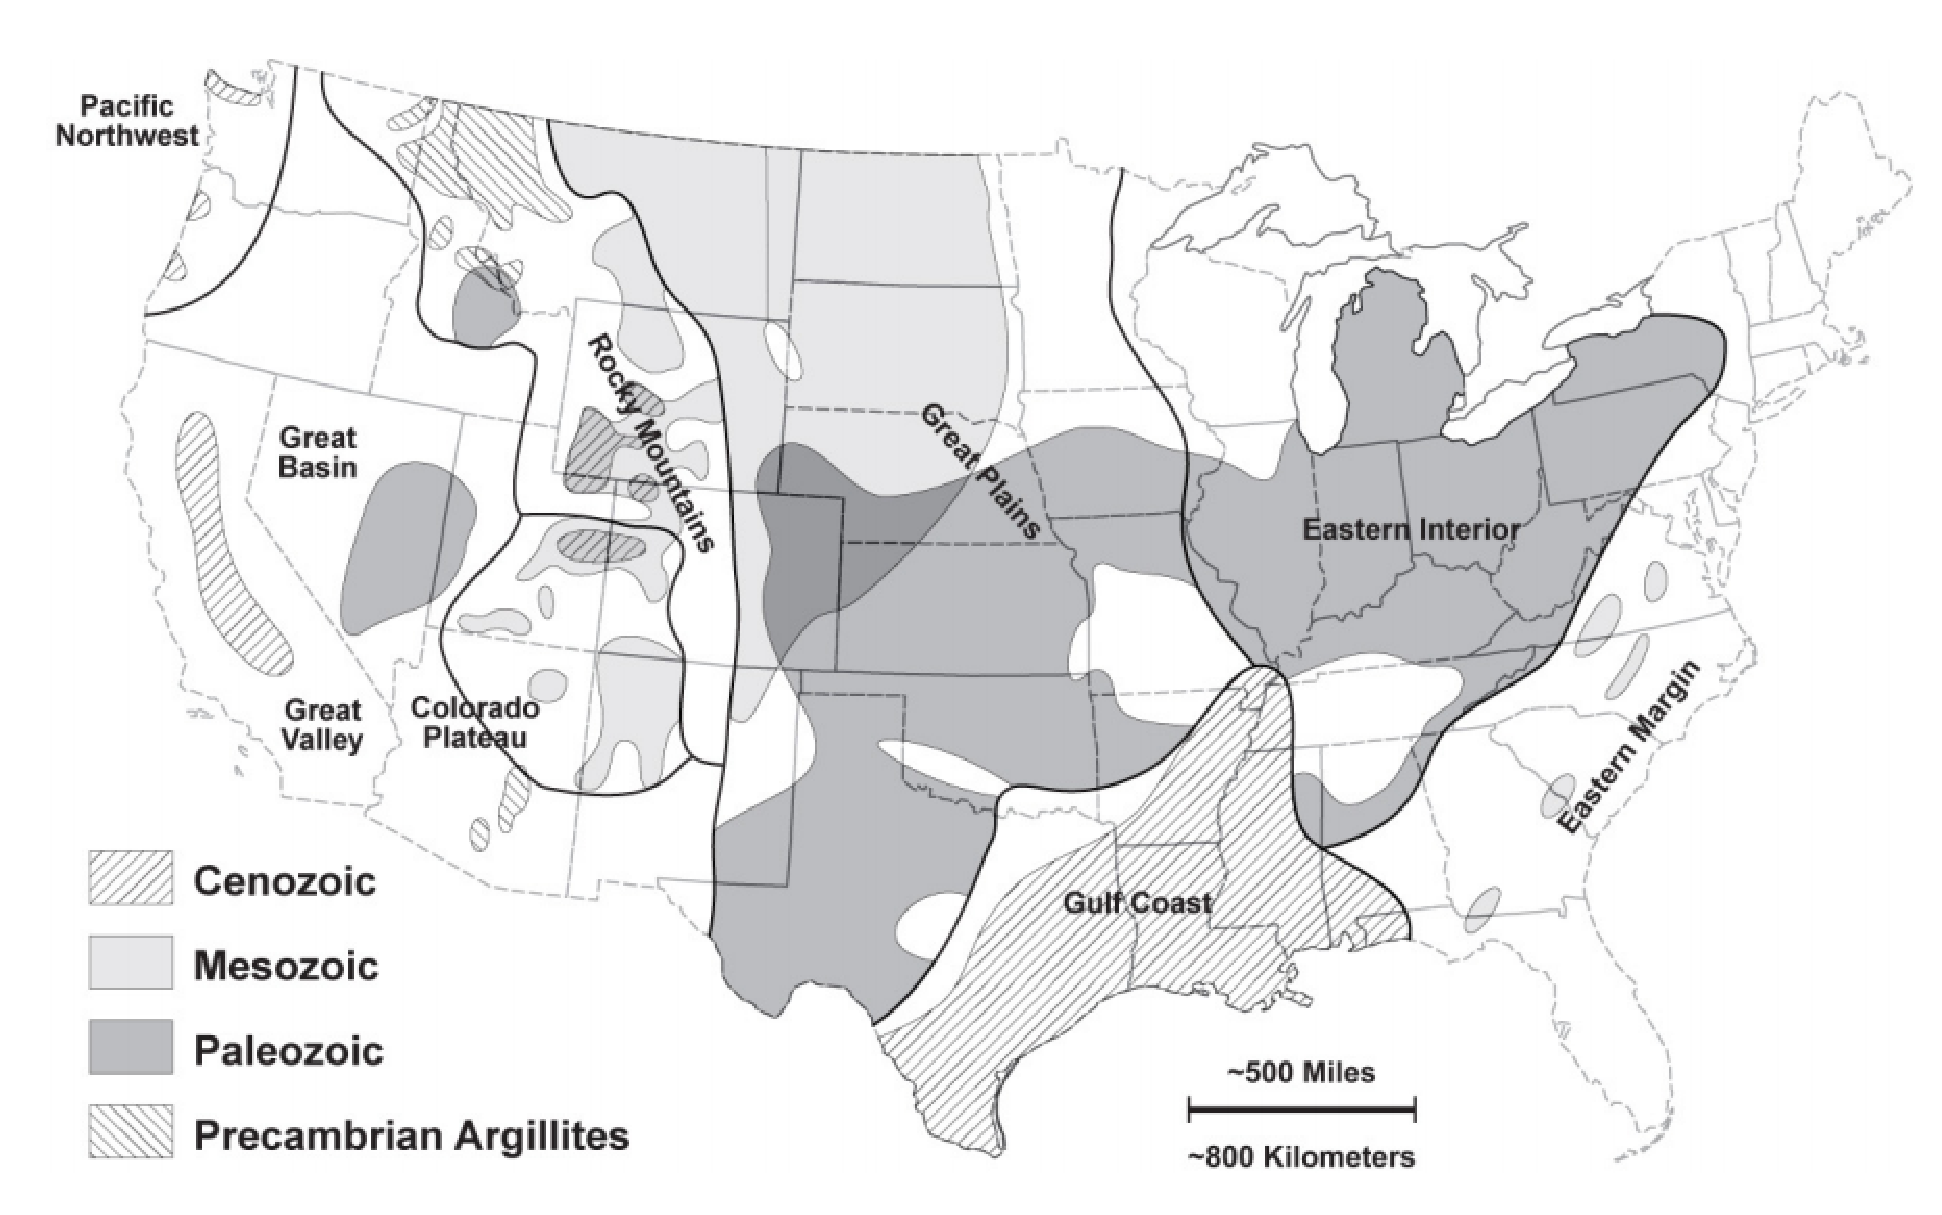
\includegraphics[width=0.8\textwidth]{clayGonzales.eps}
         \caption{U.S. Clay Deposits, ref. \cite{gonzales_shales_1985}.}
     \end{figure}
   \end{minipage}
   \hspace{0.01cm}
   \begin{minipage}{0.44\textwidth}
     \begin{figure}[h!]
         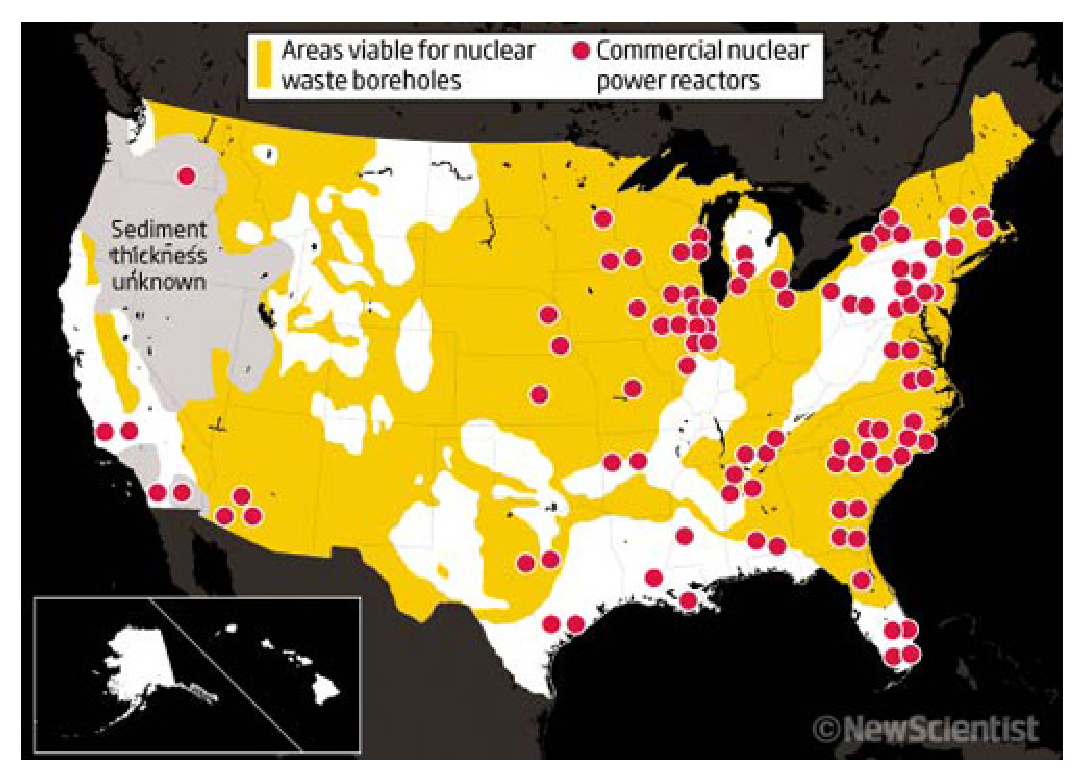
\includegraphics[width=0.8\textwidth]{boreholeNewScientist.eps}
         \caption{U.S. Crystalline Basement, ref.  \cite{newscientist_where_2011}.}
     \end{figure}
     \begin{figure}[h!]
         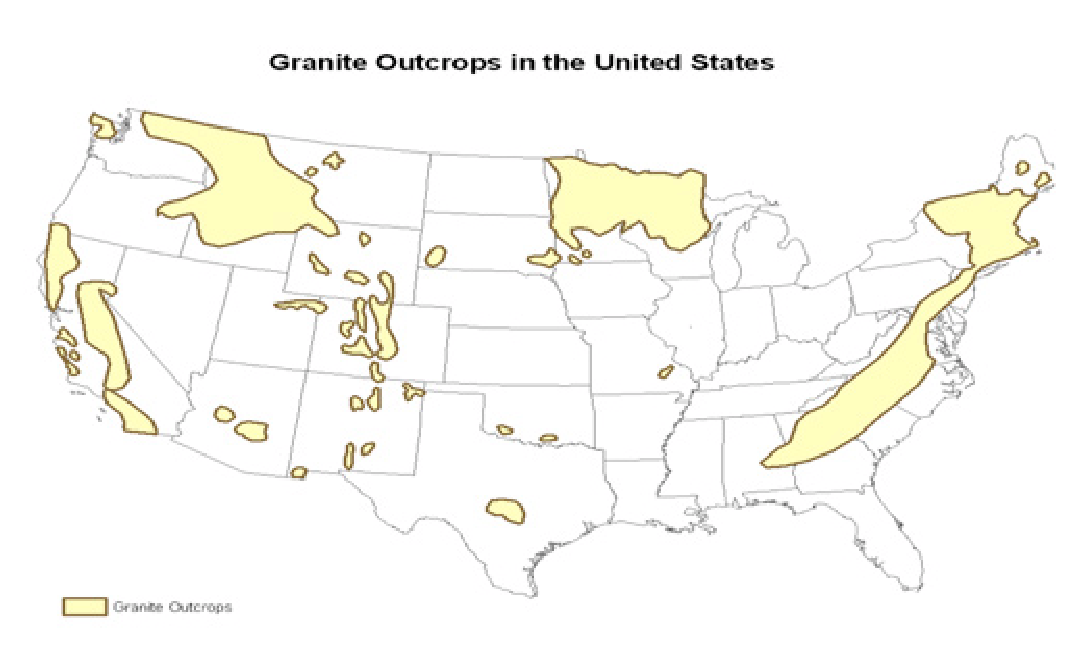
\includegraphics[width=0.8\textwidth]{graniteBush.eps}
         \caption{U.S. Granite Beds, ref. \cite{bush_economic_1976}.}
     \end{figure}
   \end{minipage}
\end{frame}


\begin{frame}[ctb!]
  \frametitle{Future Fuel Cycle Options}
   % Future Fuel Cycles
    \begin{table}
      \centering
      \footnotesize{
      \begin{tabular}{|l|l|l|}
        \multicolumn{3}{c}{\textbf{Domestic Fuel Cycle Options}}\\
        \hline
        Title & Description& Challenges \\
        \hline
        \hline
        Open          & Once Through         & High Temperatures, Volumes \\
                      & Current US PWR Fleet &      \\
                      & No Separations       &      \\
                      & No Recycling         &      \\
                      & Higher Burnups &      \\
        \hline
        Modified Open & Partial Recycling    & Both high volumes and myriad fuel streams \\
                      & Next Gen. PWR Fleet &      \\
                      & Limited Separations  &      \\
                      & Limited Transmutation &      \\
                      & Advanced Fuel Forms  &      \\
                      & HLW treatment    &          \\
        \hline
        Closed        & Full Recycling       & Myriad fuel streams \\
                      & Full Separations &      \\
                      & Full Recycling &      \\
                      & VHTGR, SFRs, &      \\
                      & other transmutation & \\
                      & HLW treatment  &      \\
        \hline
      \end{tabular}
      \caption[Fuel Cycle Options]{Domestic Fuel Cycle Options }
      \label{tab:fco}
      }
    \end{table}
\end{frame}


% layouts
% EBS choices
% Geologies


\begin{frame}[ctb!]
  \frametitle{Clay Disposal Environments}

  \begin{figure}[h!]
    \begin{center}
      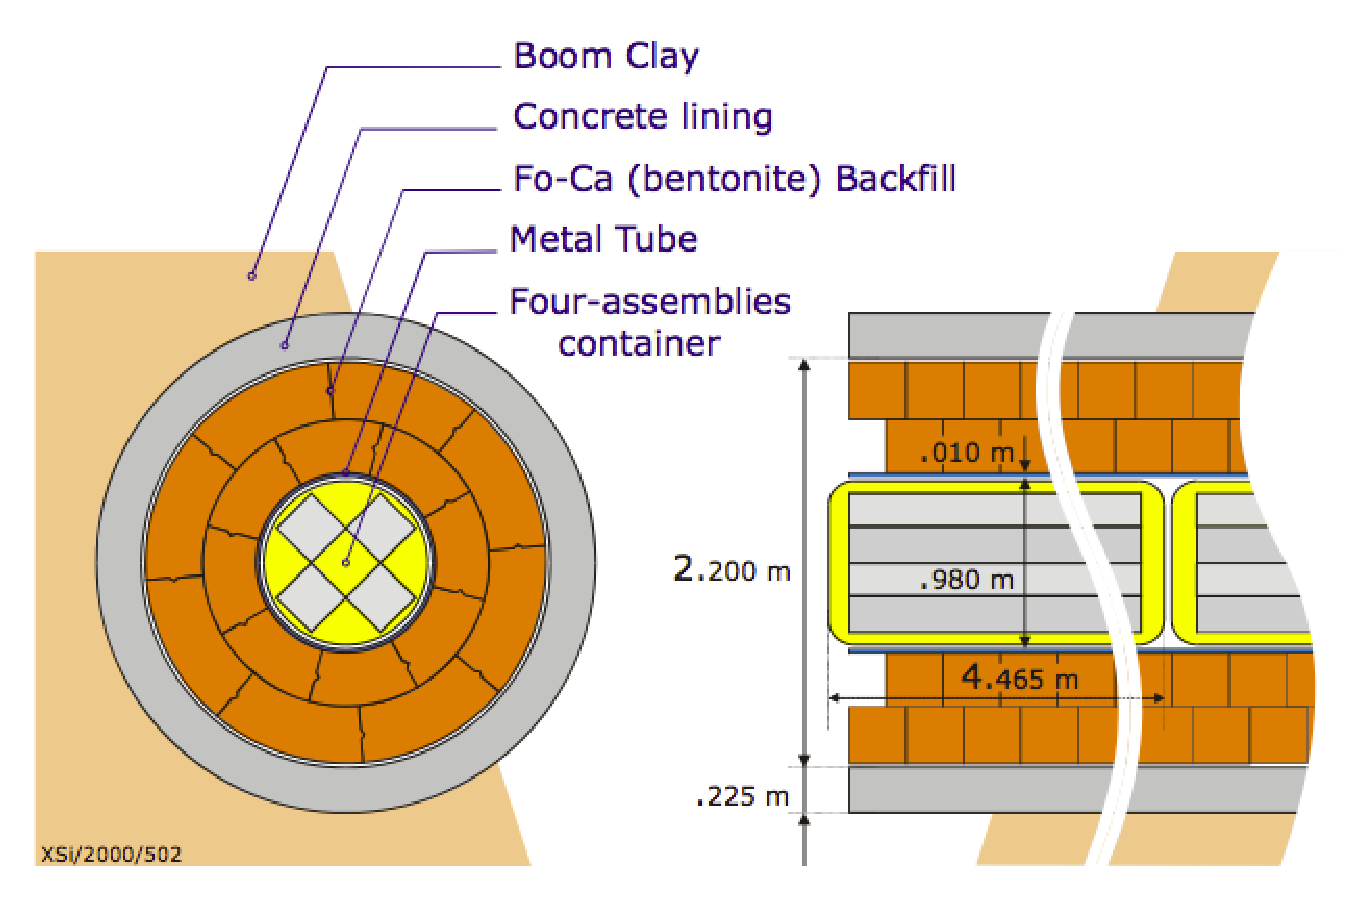
\includegraphics[height=.7\textheight]{belgianClayRedImp.eps}
    \end{center}
    \caption{Belgian reference concept in Boom Clay 
    \cite{von_lensa_red-impact_2008}.}
    \label{fig:belgianClayRedImp}
  \end{figure}

\end{frame}

\begin{frame}[ctb!]
  \frametitle{Granite Disposal Environments}

  \begin{figure}[h!]
    \begin{center}
      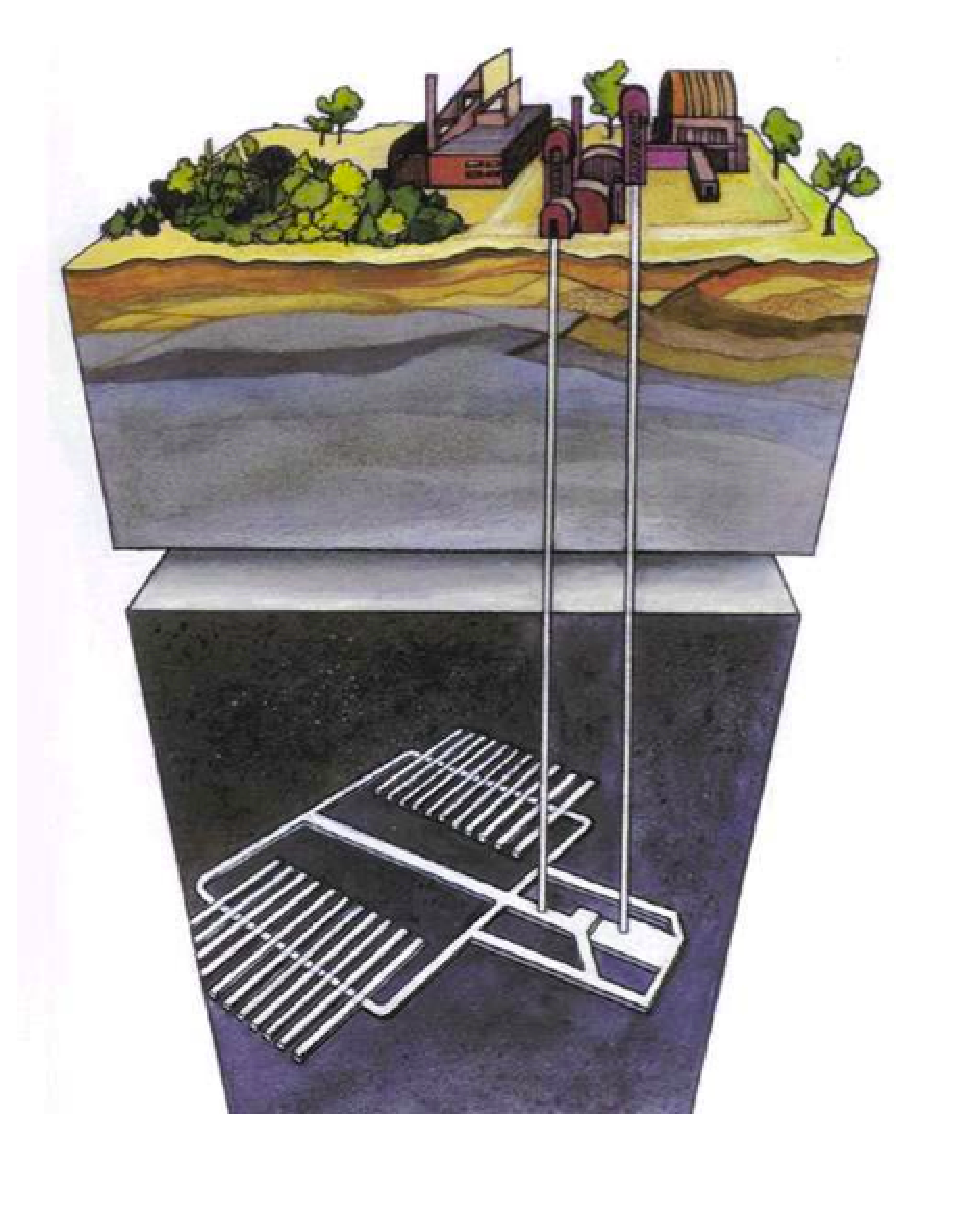
\includegraphics[height=.7\textheight]{czechGraniteRedImp.eps}
    \end{center}
    \caption{Czech reference concept in Granite 
    \cite{von_lensa_red-impact_2008}.}
    \label{fig:czechGraniteRedImp}
  \end{figure}

\end{frame}

\begin{frame}[ctb!]
  \frametitle{Salt Disposal Environments}

  \begin{figure}[h!]
    \begin{center}
      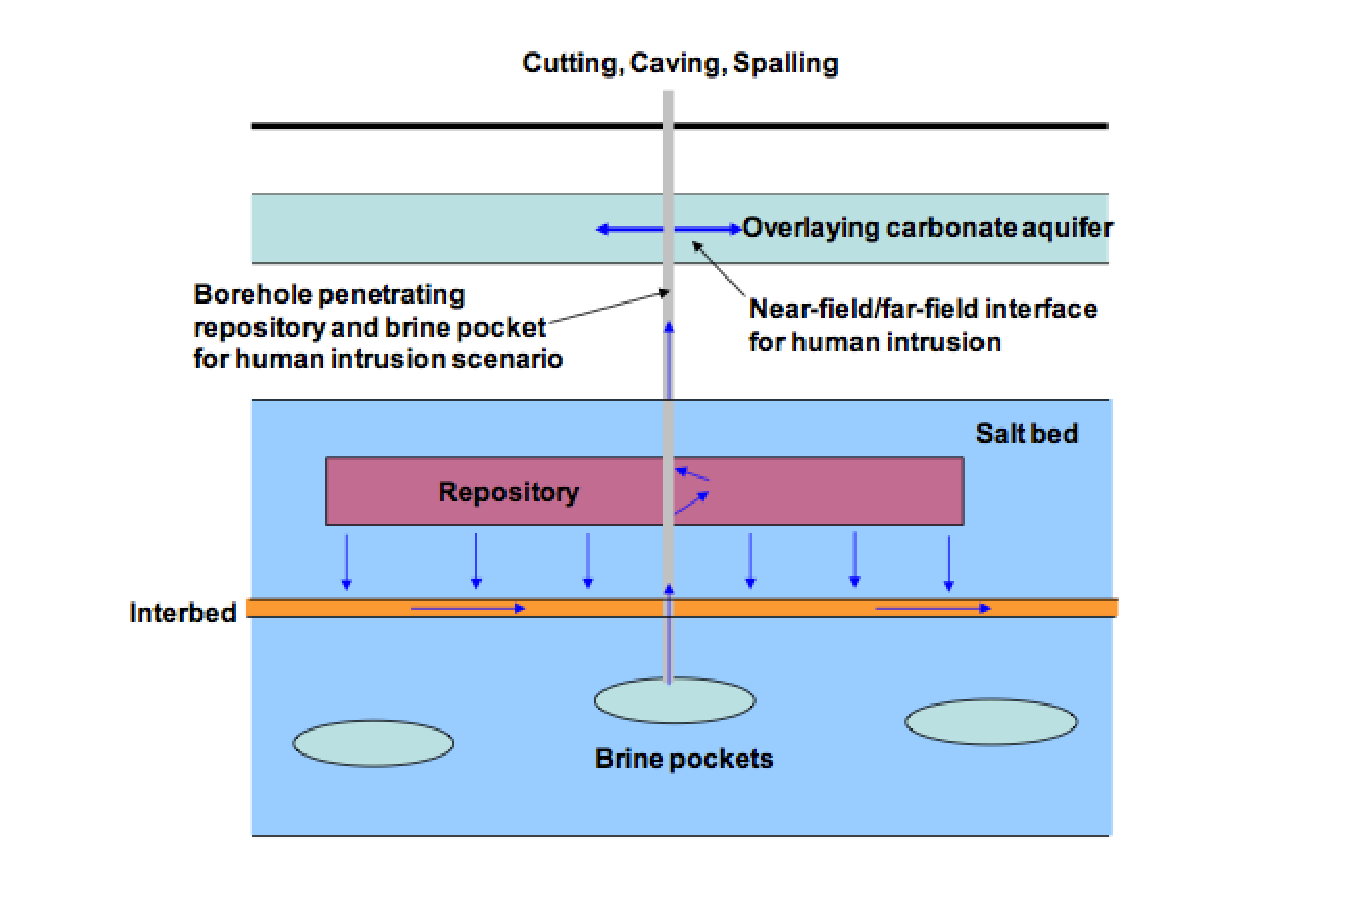
\includegraphics[height=.7\textheight]{saltGPAM.eps}
    \end{center}
    \caption{DOE-NE Used Fuel Disposition Campaign  concept in 
    Salt \cite{clayton_generic_2011}.}
    \label{fig:saltGPAM}
  \end{figure}

\end{frame}

\begin{frame}[ctb!]
  \frametitle{Deep Borehole Disposal Environment}

  \begin{figure}[h!]
    \begin{center}
      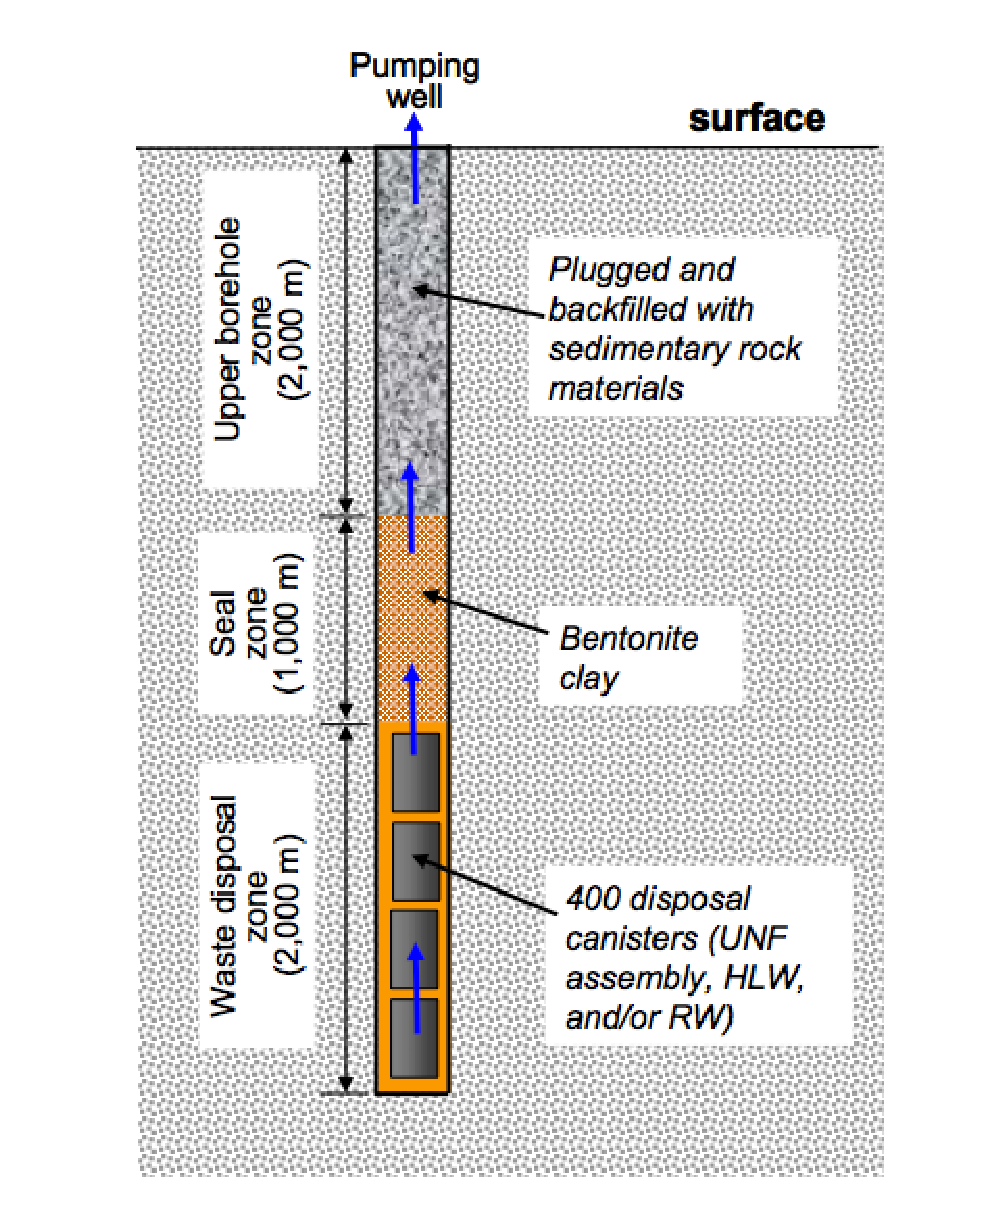
\includegraphics[height=.7\textheight]{boreholeGPAM.eps}
    \end{center}
    \caption{DOE-NE Used Fuel Disposition Campaign Deep Borehole concept 
    \cite{clayton_generic_2011}.}
    \label{fig:boreholeGPAM}
  \end{figure}

\end{frame}


\begin{frame}
  \frametitle{Repository Layouts}

  \begin{minipage}{0.49\textwidth}
    \begin{figure}[h!]
      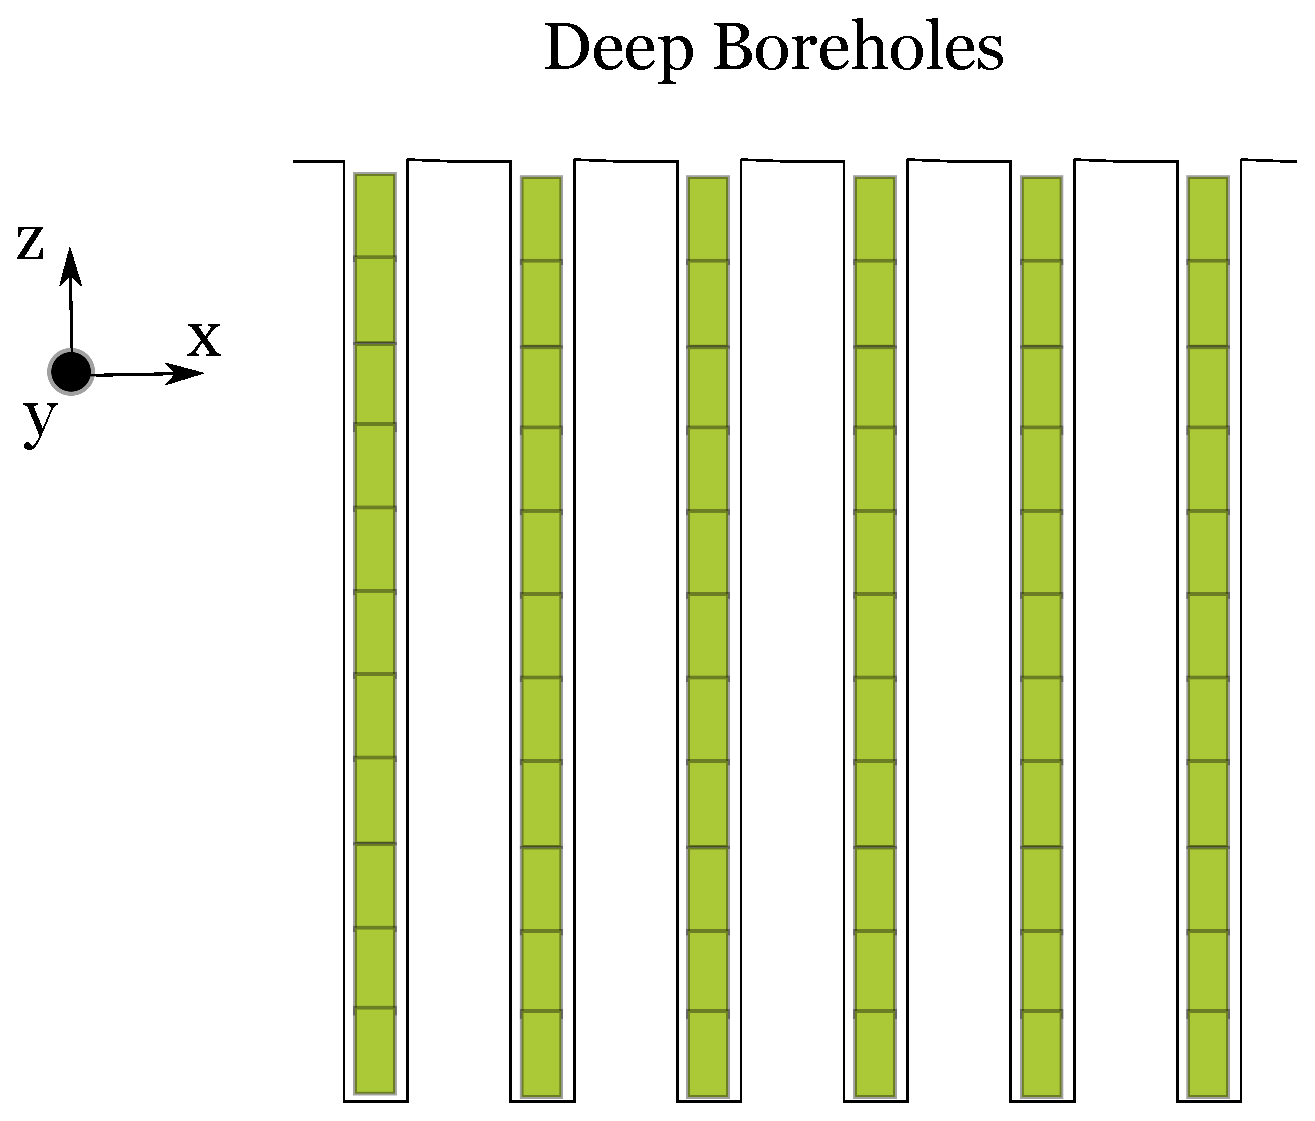
\includegraphics[width=0.75\textwidth]{boreholes.eps}
    \end{figure}
    \begin{figure}[h!]
      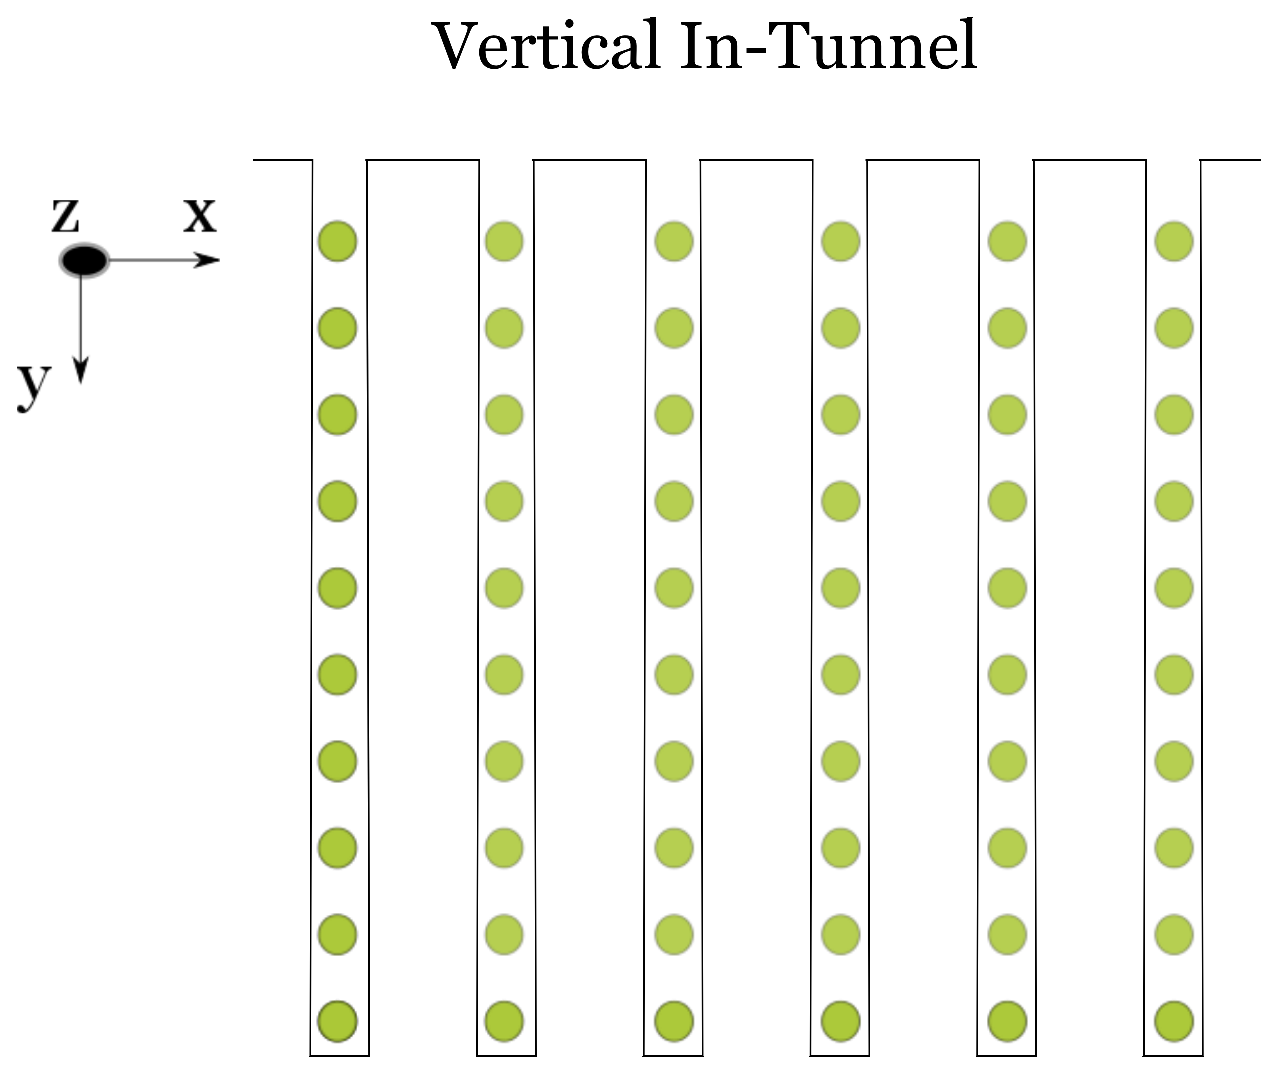
\includegraphics[width=0.75\textwidth]{vertical.eps}
    \end{figure}
  \end{minipage}
  \hspace{0.01cm}
  \begin{minipage}{0.49\textwidth}
    \begin{figure}[h!]
      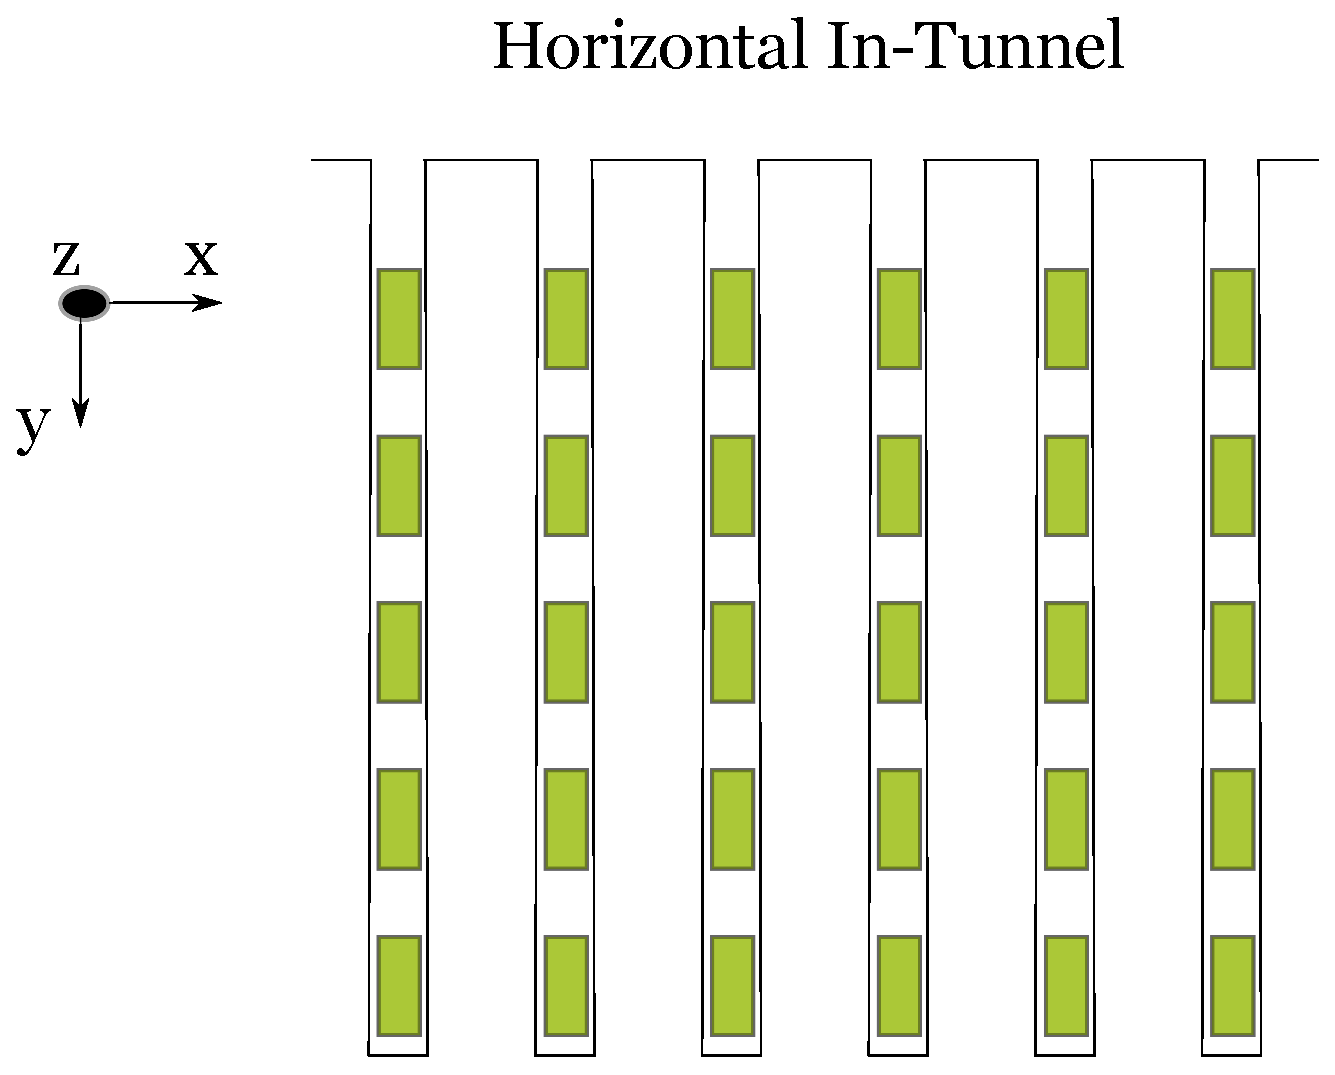
\includegraphics[width=0.8\textwidth]{horizontal.eps}
    \end{figure}
    \begin{figure}[h!]
      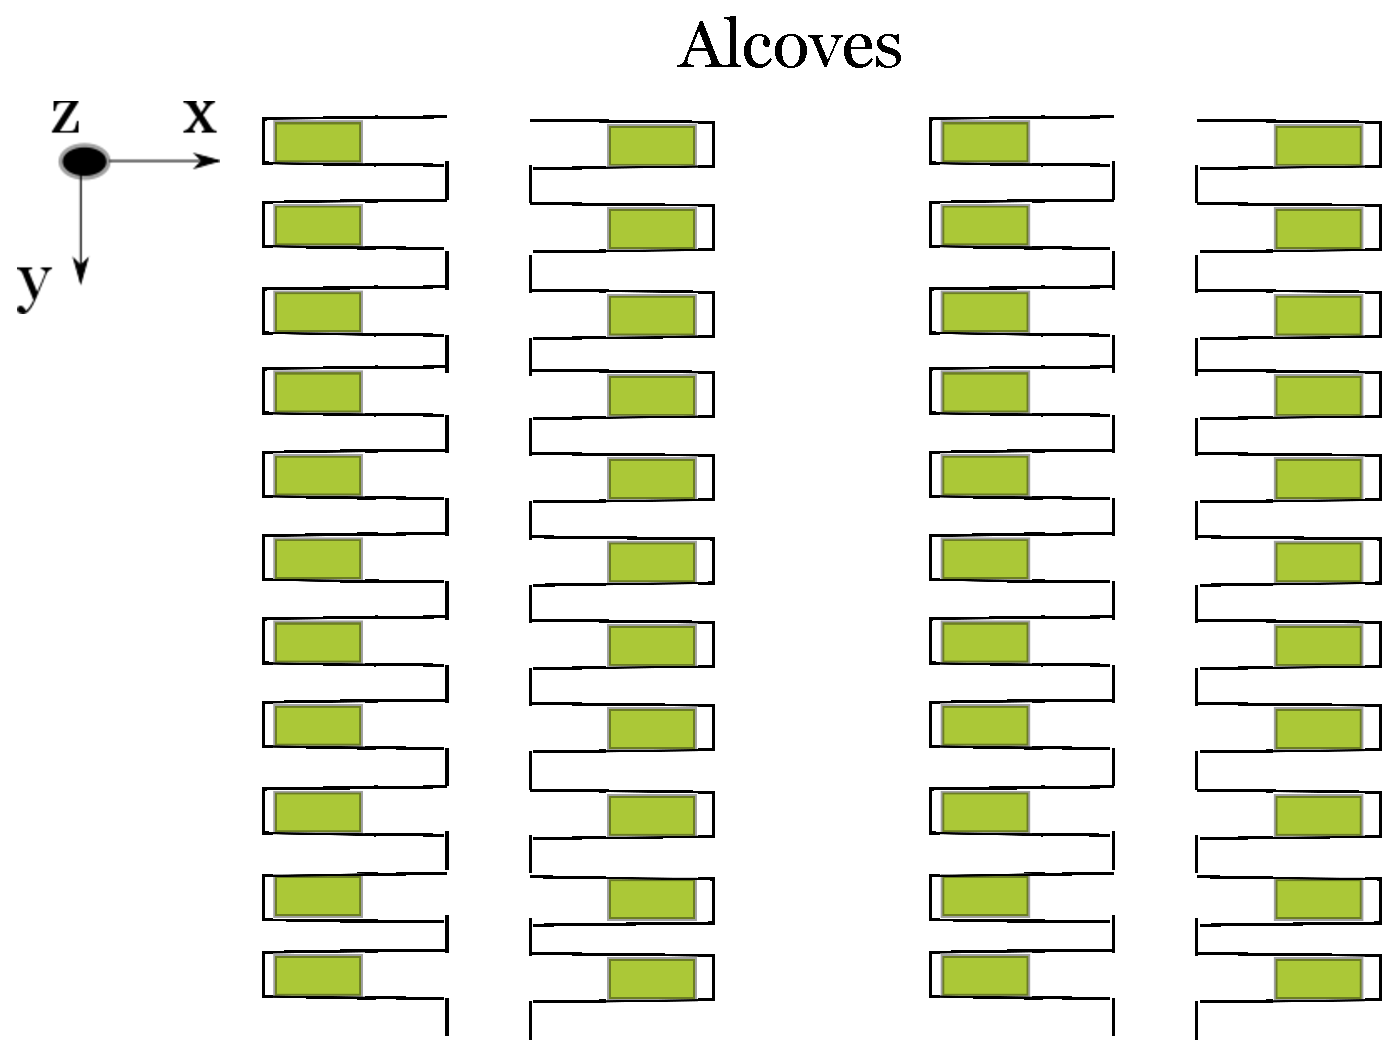
\includegraphics[width=0.8\textwidth]{alcoves.eps}
    \end{figure}
  \end{minipage}

\end{frame}
